\chapter{Evaluation}\label{C:eval}

The aim of this project was to control for and improve the repeatability, and reliability of the position and volume of the dispensed droplets on a substrate with the informed hypothesis that these are major contributors to the observed high variation in resulting the temperature evolution during the droplet's evaporation. To show the success of the project this evaluation will investigating, quantify and compare the performance and positional repeatability of the new instrumentation as well begin to as investigate its effects on the temperature evolution of the droplet's evaporation.

\section{Mechanical Stability}

Given that the express goal of this project is to produce a more stable, repeatable system for depositing droplets of a set position the mechanical stability of the instrumentation is required to be accessed and tuned to minimise vibration and pipette tip oscillations (settling time and overshoot).

To evaluate the performance of the system, a parameter sweep of the pipettes R stage motor driving settings: speed and ramp acceleration.
\subsection{Procedure}
\begin{itemize}
    \item Position tip at -1/4 revolution before zero point (proxy reservoir)
    \item Set Speed/acceleration values
    \item Swing to zero position
    \item Repeat for values across sweep: speed=1rev/s, acc=1/rev/s/s $\rightarrow$  speed=2rev/s, acc=10/rev/s/s
    \item Note: acceleration is the ramp down at end/start of motion so is what we care most about
\end{itemize}

\subsection{Results}
By taking a 25 frames per second image sequence captured via the top camera of the same automated sequence performed at various parameters the pipette tip could be motion-tracked over time to extract its relative motion frame to frame quantitatively capture the settling behaviour of the pipette tip. Minimising ensured the best chance of avoiding prematurely detachment and precise positioning at the time of dispense. 

\begin{figure}[h]
    \centering
    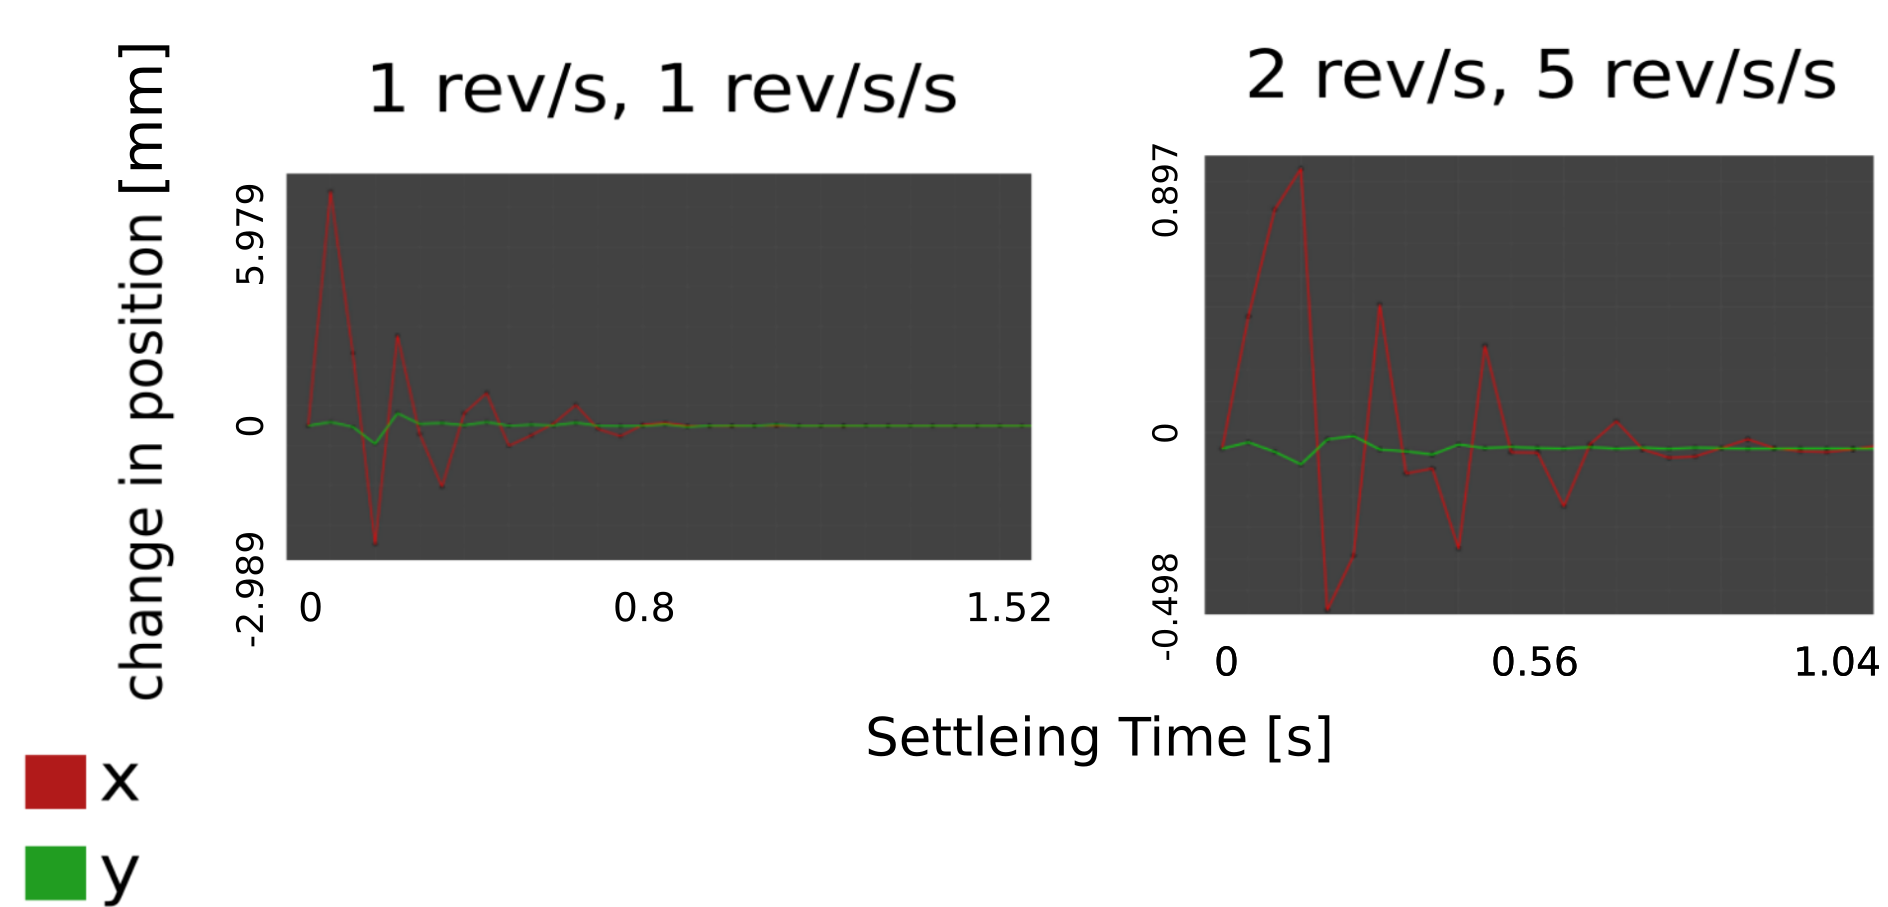
\includegraphics[width=0.5\textwidth]{img/param_sweep_osc.png}
    \caption{Worst (Left) and Best (Right) performing oscillations and settings}
    \label{Fig:tip_osc}
\end{figure}

The figure [\ref{Fig:tip_osc}] above shows this tip behaviour. This procedure and analysis helped determine a final parameter tuning for the R motor of 2 rev/s and 5 rev/s/s resulting in a maximum overshoot of 0.9mm and settling time of 1s. This can be used to inform the delay time require after tip positioning before dispensing the droplet.

\section{Droplet Volume}

Something the previous system could not achieve was accurately dispensing a variety of volumes.

\begin{wrapfigure}{r}{0.33\textwidth}
    \centering
    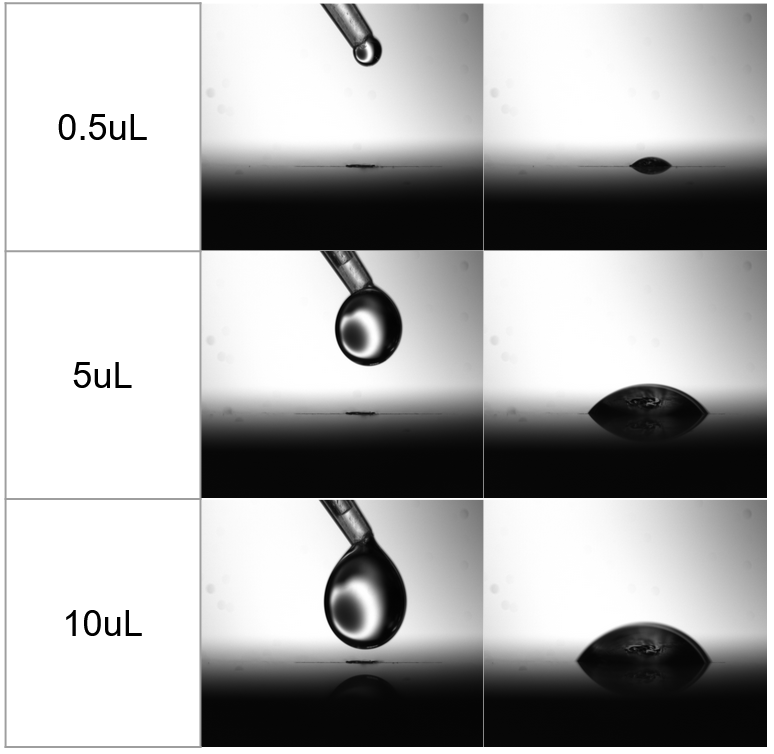
\includegraphics[width=0.3\textwidth]{img/volume_range.png}
    \caption{Successful droplet dispense and deposit of full volume range}
    \label{fig:vol_var}
\end{wrapfigure}

The use of an e-pipette eliminates variation in absolute volume to a higher precision than what this project can evaluate but additionally the use of it programmable volume feature enables this. The instrumentation however may not be able to use the full volume range of $0.5\mu L$ to $10\mu L$.

The system had been observed previously to be unable to reliably dispense above $8\mu L$ without premature detachment. This was before the Z motor coupler was refined and the motors speed adjusted.
We also had the hypothesis that variation in volume could have an effect on the y-position of the deposited droplet, via the mechanism of differing masses being affected more by surface tension with the tip.

The figure \ref{fig:vol_var}shows instrumentation successfully dispensing and depositing the full range of volumes, and confirms the systems ability to utilise the pipettes full functionality. Also of note that these results disprove the hypothesis of y-axis dependency, as after dispensing [if a delay of at least 500ms is allowed] all droplet volumes hang and settle with gravity.  

To ensure consistent performance over the volume range the Z-height dip must be varied to successfully deposit the droplet on the substrate and prevent overly deforming it at high volume.

\begin{figure}[h]
    \centering
    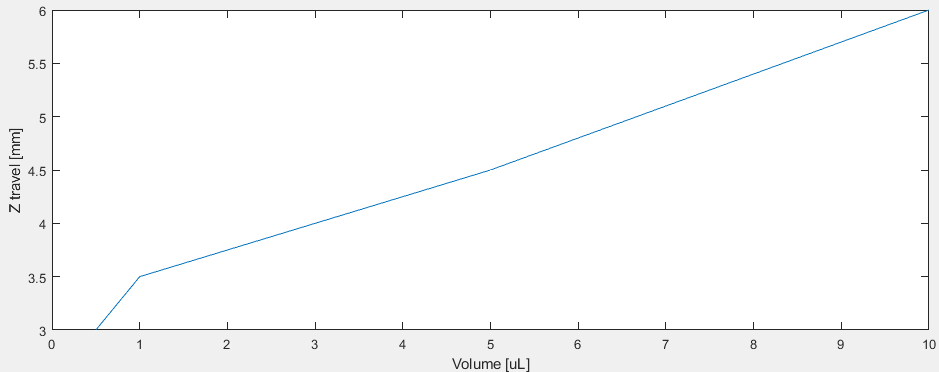
\includegraphics[width=0.5\textwidth]{img/vol_z.png}
    \caption{Drop Volume vs Required Z travel}
\end{figure}

\section{Repeatability and Reliability}

This section aims to produce the main set of comparable results for evaluating the projects produced system against the output of the previous setup. Thus justifying the success of one of main goals.

\subsection{Procedure}
\begin{itemize}
    \item \textbf{Initial Setup:} Roughly Position substrate stage, reservoir platform and note angular positions as well as vertical clearance requirements.
    \item \textbf{Zero System:} Using overhead camera precisely position pipette tip above substrate centre
    \item \textbf{Data Acquisition:} Initialise cameras, collect pixel:mm calibration data for analysis, initial LabView temperature logger, and environmental monitor noted. Info: temperature data rate, camera frame rate
    \item \textbf{Automated Sequence:} Via the serial link, enter the procedures command sequence to represent $\rightarrow$ lower, draw up fluid, raise, position over the substrate, dispense, lower, raise, clear camera view. With appropriate delays.
    \item \textbf{Capture:} Begin data collection and automated dispense.
    \item \textbf{Repeat: } 3 times. Each time carefully cleaning substrate surface to minimised up measured factors.
\end{itemize}

\subsection{Analysis and Results}
To show the system successfully increases the consistency of droplet position and investigate whether this supports the hypothesis that this resulted in better temperature consistency.

\subsection{Position}

The main bulk of the design and effort of this project were put towards ensuring consistent, accurate and repeatable pipette tip positioning with the intention of greatly decrease the run to run variance in droplet position. This was due to the static point temperature measurement being taken by a thermocouple and initial evaluation indicating a correlation between droplet offset from thermocouple position and temperature data variation.

\begin{figure}[h]
    \centering
    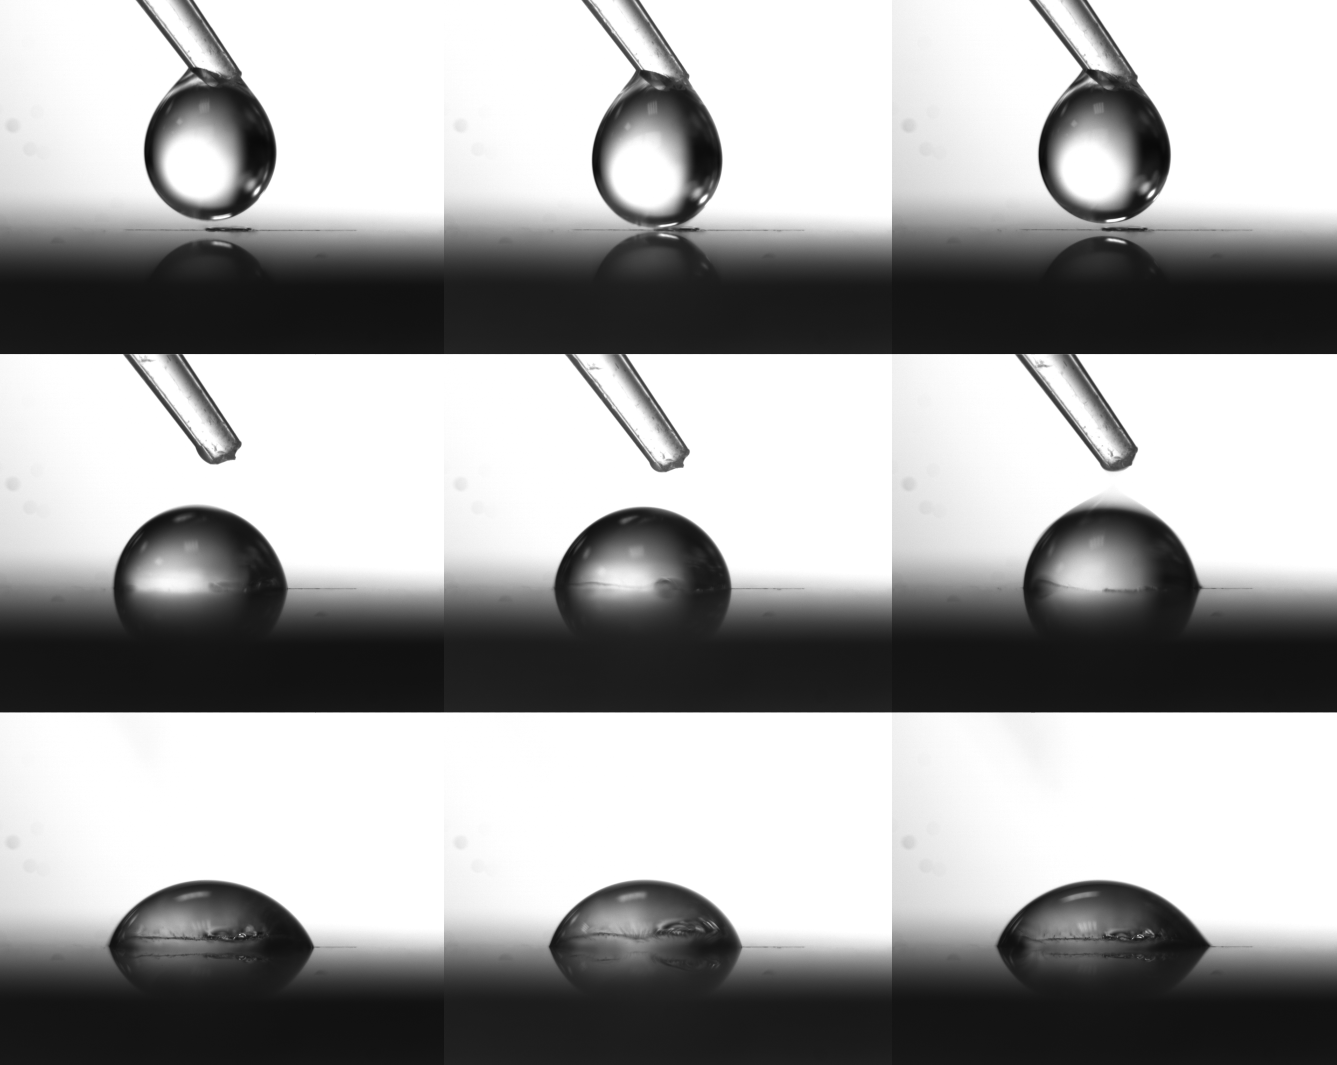
\includegraphics[width=0.4\textwidth]{img/side_drops.png}
    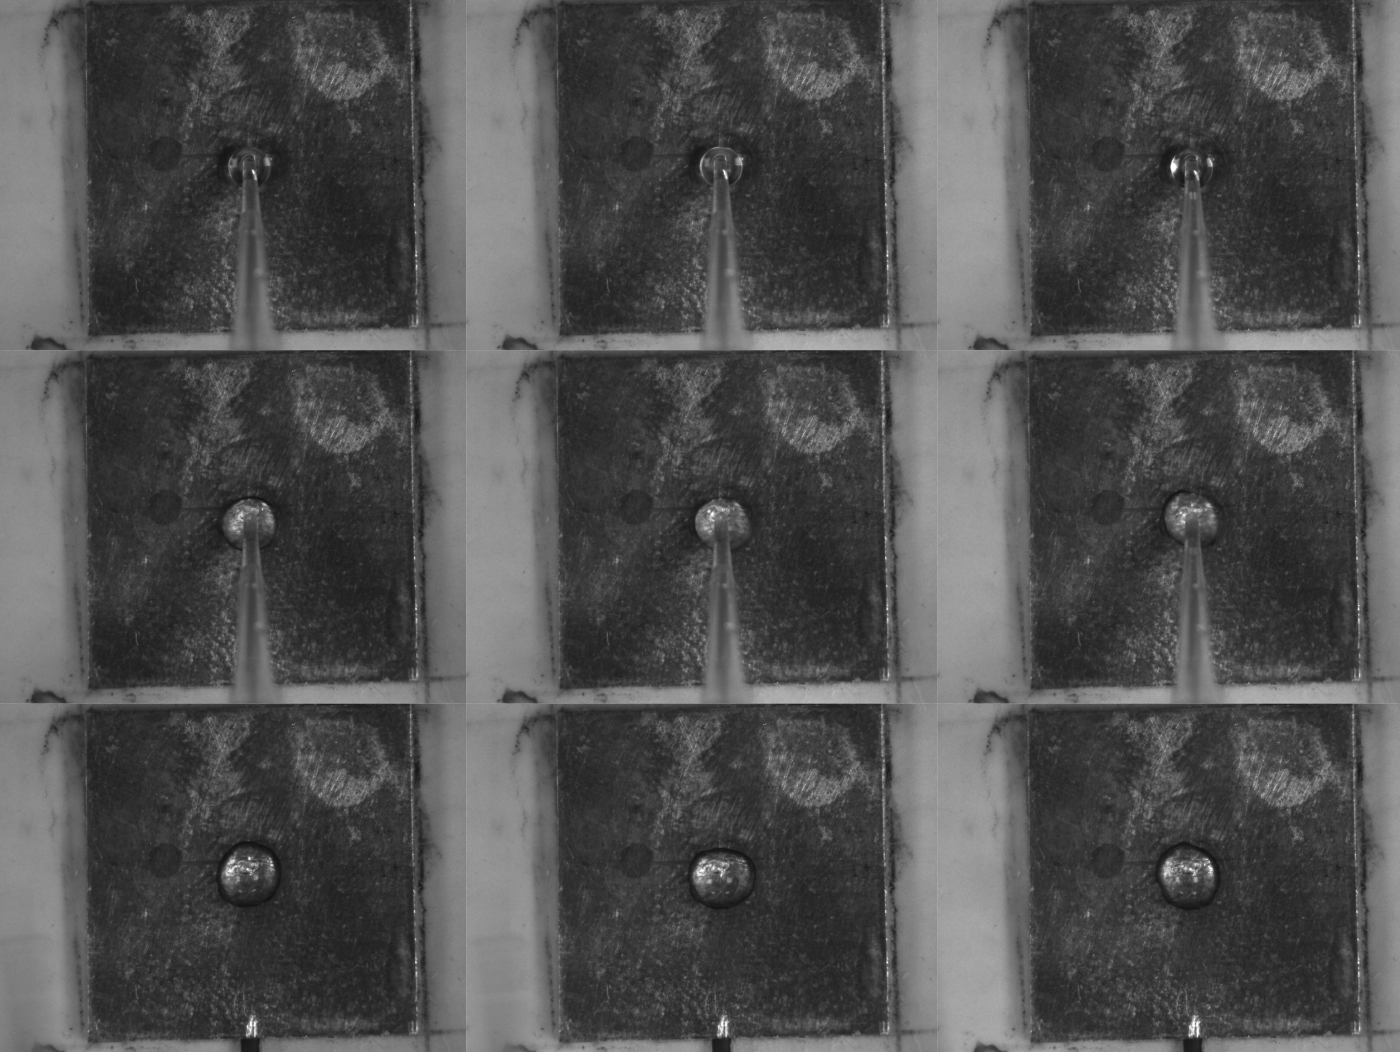
\includegraphics[width=0.4\textwidth]{img/top_drops.png}
    \caption{Visual results of consecutive experimental runs (Runs are column-wise)}
    \label{fig:drops_eval}
\end{figure}

Prior sections have covered to tuning and design decisions taken to produce consist pipette tip position but how does this translate to droplet variation. Figure  \ref{fig:drops_eval}shows the qualitative results of 3 consecutive 10 $\mu L$ experiments. By observing these results, the pipette tip placement is indistinguishable between runs and hanging droplets before contact are also consistent. This image data formed the basis for further analysis to extract quantitative information.

Collected calibration reference images allows the translation of pixels to mm, and using an image processing and analysis tool droplet centre offset from substrate centre as well as surface contact area measured to quantify performance for comparison to initial system.

\begin{figure}[h]
    \centering
    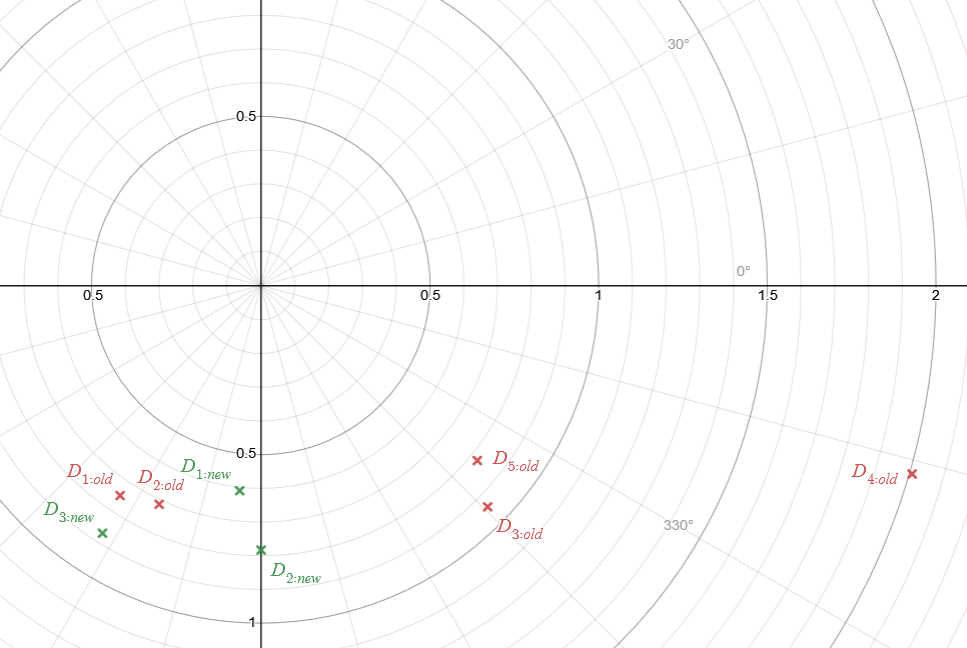
\includegraphics[width=0.5\textwidth]{img/pos_comp.png}
    \caption{Caparison of old (red) and new (green) droplet positions}
\end{figure}

\subsection{Temperature Evolution}

The above droplet runs were also accompanied by the collection of substrate temperature data via the embedded thermocouple. The thermocouple was read at 30Hz, and MatLab was used to postprocess and analyse the data. As a pre-processing step a 1sec rolling average is applied to the collected vectors. They are then time aligned to zero at the point of droplet contact, indicated by sudden temperature drop. This The data is then transformed into a temperature delta relative to the temperature just before contact. 

\begin{figure}[h]
    \centering
    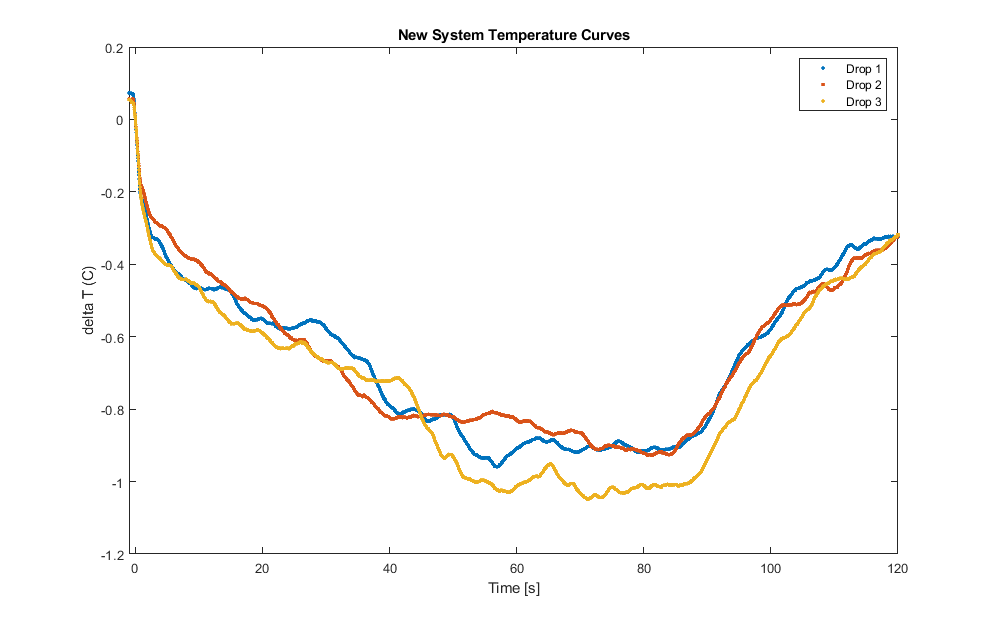
\includegraphics[width=0.5\textwidth]{img/new_temp.png}
    \caption{Captured Temperature Evolution of new drop tests}
\end{figure}

It is worth noting that this temperature data is in no way comprehensive, and differs from the initial data due to a difference in substrate material: stainless steel vs copper. 

\subsection{Summery}

\begin{table}[h]
    \centering
    \begin{tabular}{|l|l|l|l|}
    \hline
             & Pos Offset {[}mm{]} & delta T {[}c{]} & contact area ($mm^2$)  \\ \hline
    Drop 1   & 0.6126              & -0.9044         & 15.8928                               \\ \hline
    Drop 2   & 0.7856              & -0.9238         & 15.7082                               \\ \hline
    Drop 3   & 0.8728              & -1.009          & 15.0274                               \\ \hline
    Variance & 0.01753948          & 0.003096        & 0.20774716   \\ \hline
    \end{tabular}
    \end{table}

